% SC2008 — Chapter 3: Transport — UDP, rdt, Go-Back-N (0->100 ground-up)
\chapter{Transport Layer: UDP and Reliable Data Transfer}
\label{ch:transport-udp}

\begin{quote}
\emph{``The network promised to try its best, but trying is not delivering.''} --- Reliable transfer is the engineering answer to an unreliable world: we add numbers, timers, and retransmissions until loss, corruption, and delay become invisible to the application.
\end{quote}

\noindent\fbox{\parbox{\dimexpr\linewidth-2\fboxsep-2\fboxrule}{%
\textbf{From zero: no transport background assumed.} We start from the idea that the network layer delivers datagrams that may be lost or corrupted, then build up in steps: why ports exist, what UDP adds, and how to create reliability from scratch---acknowledgments, sequence numbers, timers---culminating in pipelined Go-Back-N. Pictures first, then formalism.}}
\vspace{0.4em}

\section*{Learning Outcomes}
After this chapter you will be able to:
\begin{enumerate}[label=(L\arabic*)]
    \item explain multiplexing/demultiplexing and why transport needs port numbers;
    \item describe the UDP segment format, checksum computation, and its use cases;
    \item design stop-and-wait reliable transfer over a lossy/corrupt channel using sequence numbers, ACKs, and timers;
    \item analyse Go-Back-N with its sliding window, cumulative ACKs, and utilization;
    \item compare Go-Back-N versus Selective Repeat and compute efficiency.
\end{enumerate}

% ============================================================
\section{Why a Transport Layer?}
\label{sec:why-transport}
An application writes bytes; the network moves datagrams between hosts. The IP layer gets a packet \emph{to the right house}, but which \emph{person inside} should receive it? The transport layer adds \emph{ports}---16-bit mailboxes---so multiple processes on one host can share the network safely.

\emph{Intuition.} Think of an apartment block (host) with one street address (IP). The lobby sorts letters by apartment number (port). Two apps---browser and DNS resolver---are two apartments sharing the same address. The operating system is the sorter.

Formally, \emph{multiplexing} gathers data from sockets into segments at the sender; \emph{demultiplexing} delivers arriving segments to the correct socket by destination port (and, for TCP, the 4-tuple). UDP demultiplexes by destination IP and port only; TCP uses source IP/port as well.

\begin{figure}[h]\centering
\begin{tikzpicture}[scale=0.74,every node/.style={font=\scriptsize}]
\node[draw,thick,rounded corners=3pt,fill=blue!12,minimum width=2.4cm,minimum height=1.0cm,align=center] (app1) at (0,2.2) {Browser\\{\tiny port 54321}};
\node[draw,thick,rounded corners=3pt,fill=green!15,minimum width=2.4cm,minimum height=1.0cm,align=center] (app2) at (0,0.7) {DNS client\\{\tiny port 5353}};
\node[draw,thick,rounded corners=3pt,fill=orange!15,minimum width=2.6cm,minimum height=1.1cm,align=center] (sock) at (3.8,1.45) {Transport\\{\tiny UDP / TCP}};
\node[draw,thick,rounded corners=3pt,fill=violet!12,minimum width=2.6cm,minimum height=1.0cm,align=center] (ip) at (7.6,1.45) {Network (IP)\\{\tiny to host}};
\draw[-{Latex},thick,blue!60!black] (app1) -- (sock) node[midway,above,font=\tiny] {socket};
\draw[-{Latex},thick,blue!60!black] (app2) -- (sock);
\draw[-{Latex},thick,blue!60!black] (sock) -- (ip) node[midway,above,font=\tiny] {segment};
\node[draw,thick,fill=yellow!12,rounded corners=2pt,inner sep=2pt,font=\tiny,align=center] at (3.8,-0.55) {Port = apartment number\\IP = building address};
\end{tikzpicture}
\caption{Demultiplexing intuition: IP gets the datagram to the host; port delivers it to the right socket. UDP keys on (dest IP, dest port).}
\label{fig:demux}
\end{figure}

% ============================================================
\section{UDP: Do Almost Nothing, Do It Fast}
\label{sec:udp}
\emph{User Datagram Protocol} adds exactly two things to IP: ports and an optional checksum. No handshake, no reliability, no ordering, no congestion control---just a thin wrapper.

\begin{figure}[h]\centering
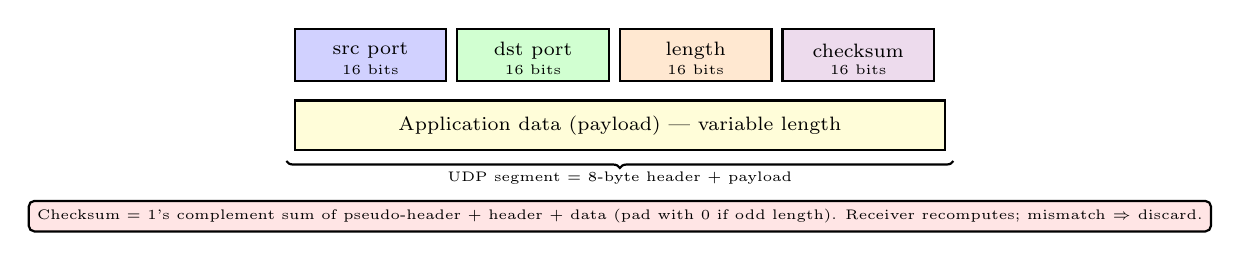
\begin{tikzpicture}[scale=0.70,every node/.style={font=\scriptsize}]
\foreach \i/\txt/\col in {0/src port/blue!18,1/dst port/green!18,2/length/orange!18,3/checksum/violet!14} {
  \pgfmathsetmacro{\x}{\i*2.95}
  \draw[thick,fill=\col] (\x,0) rectangle (\x+2.75,0.95);
  \node[align=center,font=\scriptsize] at (\x+1.375,0.55) {\txt};
  \node[font=\tiny] at (\x+1.375,0.20) {16 bits};
}
\node[font=\tiny,align=center] at (5.85,-0.55) {Header = 8 bytes total};
\draw[thick,fill=yellow!15] (0,-1.25) rectangle (11.8,-0.35);
\node[font=\scriptsize,align=center] at (5.9,-0.80) {Application data (payload) --- variable length};
\draw[decorate,decoration={brace,mirror},thick] (-0.15,-1.45)--(11.95,-1.45) node[midway,below,font=\tiny] {UDP segment = 8-byte header + payload};
\node[draw,thick,fill=red!10,rounded corners=2pt,inner sep=3pt,font=\tiny,align=left] at (5.9,-2.45) {Checksum = 1's complement sum of pseudo-header + header + data (pad with 0 if odd length). Receiver recomputes; mismatch $\Rightarrow$ discard.};
\end{tikzpicture}
\caption{UDP segment format. Four 16-bit fields then payload. The simplicity is the point: minimal overhead, minimal guarantees.}
\label{fig:udp-format}
\end{figure}

\paragraph{Checksum.} Sender sums 16-bit words (including a pseudo-header with IP addresses), takes ones' complement, and stores it. Receiver repeats the sum including the checksum---result \texttt{0xFFFF} means no detected error. It is a \emph{detection} code, not correction. Formally,
\begin{equation}
\text{checksum}=\sim\sum_{\text{16-bit words}} w_i \quad\text{(ones' complement arithmetic).}
\end{equation}
If any bit flips, the sum changes with high probability, and the datagram is silently dropped.

\paragraph{When UDP?} DNS lookups (one query, one reply; retries are cheap), DHCP, SNMP, QUIC's underlay, real-time media where a late retransmission is useless, and any protocol that implements its own reliability above UDP.

\begin{lstlisting}[language=Python]
import socket
# UDP client: no connection, just sendto / recvfrom
sock = socket.socket(socket.AF_INET, socket.SOCK_DGRAM)
sock.sendto(b"hello udp", ("8.8.8.8", 53))
data, addr = sock.recvfrom(512)   # may be lost -- caller must retry
print(f"got {len(data)} bytes from {addr}")
# checksum is computed by OS/kernel; app sees only success or timeout
\end{lstlisting}

% ============================================================
\section{Reliable Data Transfer: Building Reliability from Nothing}
\label{sec:rdt}
The lower layer is \emph{unreliable}: bits may flip, packets may be lost, order may shuffle, and delay may be unbounded. We successively strengthen the service.

\paragraph{rdt 1.0: reliable channel.} Trivial---just send. Assumes perfection; useless in practice but fixes the API.

\paragraph{rdt 2.x: bit errors, no loss.} Add \emph{ACK} (positive) and \emph{NAK} (negative). Sender waits for feedback. Problem: ACK/NAK can themselves be corrupted. Fix: number packets $0,1$ alternating and ACK the sequence. rdt~2.1 uses ACK/NAK; rdt~2.2 uses ACKs only with duplicate-ACK meaning ``please resend.''

\paragraph{rdt 3.0: errors plus loss.} Add a \emph{countdown timer}. If no ACK arrives before timeout, retransmit. The receiver discards duplicates by checking the sequence number. This is \emph{stop-and-wait}: one packet in flight at a time.

\begin{definition}[Stop-and-wait invariant]
Sender has at most one unacknowledged packet with sequence $s\in\{0,1\}$. Receiver expects $r\in\{0,1\}$. On data with $s=r$, deliver and flip $r$; otherwise resend ACK$_r$.
\end{definition}

Utilization reveals the flaw. Let $L$ be bits per packet, $R$ the link rate, $RTT$ the round trip, and $d_{\text{trans}}=L/R$. Then
\begin{equation}
U_{\text{stop-wait}}=\frac{d_{\text{trans}}}{d_{\text{trans}}+RTT}
=\frac{L/R}{L/R+RTT}\approx \frac{L}{R\cdot RTT}\quad\text{when }L/R\ll RTT.
\end{equation}
For $L=10^4$ bits, $R=1$ Gbps, $RTT=30$ ms, $U\approx 0.03\%$---the link idles while waiting.

\begin{lstlisting}[language=Python]
def checksum16(data: bytes) -> int:
    """Ones' complement 16-bit checksum (UDP-style, simplified)."""
    if len(data) % 2 == 1:
        data += b"\x00"
    s = sum(int.from_bytes(data[i:i+2], "big") for i in range(0, len(data), 2))
    while s >> 16:          # fold carry
        s = (s & 0xFFFF) + (s >> 16)
    return (~s) & 0xFFFF

def rdt_send(sock, payload: bytes, addr, seq: int, timeout=0.5):
    """Stop-and-wait send with seq 0/1 and retransmission on timeout."""
    import socket as sk
    sock.settimeout(timeout)
    pkt = seq.to_bytes(1, "big") + payload
    while True:
        sock.sendto(pkt, addr)
        try:
            ack, _ = sock.recvfrom(1024)
            if ack and ack[0] == seq:   # correct ACK
                return seq ^ 1          # next sequence
        except sk.timeout:
            continue                    # retransmit
\end{lstlisting}

% ============================================================
\section{Pipelining and Go-Back-N}
\label{sec:gbn}
To fill the pipe, allow $N$ unacknowledged packets. Sliding windows give three ideas: sequence numbers $0\ldots 2^k-1$, a \emph{send window} $[base, base+N-1]$, and \emph{cumulative ACKs} (ACK $n$ means ``all $ \le n$ received'').

\begin{figure}[h]\centering
\begin{tikzpicture}[scale=0.66,every node/.style={font=\scriptsize}]
% timeline GBN with loss
\draw[thick,->] (0,0) -- (0,-5.6) node[below,font=\tiny] {time $\downarrow$};
\draw[thick,->] (6.5,0) -- (6.5,-5.6) node[below,font=\tiny] {time $\downarrow$};
\node[font=\footnotesize\bfseries,fill=blue!10,rounded corners=2pt,inner sep=2pt] at (0,0.35) {Sender (window $N=4$)};
\node[font=\footnotesize\bfseries,fill=green!10,rounded corners=2pt,inner sep=2pt] at (6.5,0.35) {Receiver};
% packets
\foreach \i/\y in {0/0.0,1/-0.7,2/-1.4,3/-2.1} {
  \pgfmathsetmacro{\seq}{\i}
  \draw[-{Latex},thick,blue!60!black] (0.4,\y-0.15) -- (6.1,\y-0.55) node[midway,above,font=\tiny,fill=white,inner sep=1pt] {pkt \seq};
}
% pkt2 lost -> X
\draw[thick,red!70!black] (3.1,-1.85) -- (3.6,-2.15); \draw[thick,red!70!black] (3.1,-2.15) -- (3.6,-1.85);
\node[font=\tiny,red!70!black,fill=red!5,rounded corners=1pt,inner sep=1pt] at (3.35,-2.45) {loss};
% ACKs for 0,1 arrive
\draw[-{Latex},thick,green!50!black] (6.1,-0.95) -- (0.4,-1.35) node[midway,above,font=\tiny,fill=white,inner sep=1pt] {ACK 0};
\draw[-{Latex},thick,green!50!black] (6.1,-1.65) -- (0.4,-2.05) node[midway,above,font=\tiny,fill=white,inner sep=1pt] {ACK 1};
% dup ACK1 for pkt3 (out of order discarded)
\draw[-{Latex},thick,orange!70!black,dashed] (6.1,-2.75) -- (0.4,-3.15) node[midway,above,font=\tiny,fill=white,inner sep=1pt] {ACK 1 (dup)};
% timeout then GBN retransmits 2,3,4,5
\draw[thick,red!60!black,dashed] (0.2,-3.55) rectangle (2.4,-4.05);
\node[font=\tiny,red!60!black,align=center] at (1.3,-3.80) {timeout};
\foreach \i/\y in {2/-4.20,3/-4.60,4/-5.00} {
  \draw[-{Latex},thick,blue!60!black] (0.4,\y) -- (6.1,\y-0.30) node[midway,above,font=\tiny,fill=white,inner sep=1pt] {pkt \i};
}
\node[draw,fill=yellow!10,rounded corners=2pt,font=\tiny,align=left,inner sep=3pt] at (3.25,-5.75) {GBN rule: on timeout, resend \emph{all} $N$ unACKed from base. Receiver keeps only in-order; out-of-order $\Rightarrow$ discard + dup ACK.};
\end{tikzpicture}
\caption{Go-Back-N ($N=4$) time-line: pipelined sends, loss of pkt 2, cumulative ACKs, and timeout-driven retransmission of the whole window. Window slides only when base is ACKed.}
\label{fig:gbn}
\end{figure}

\paragraph{Window mechanics.} Sender keeps $base$, $nextseqnum$, and a timer for $base$. Receiver expects $expectedseqnum$. On correct in-order arrival, deliver and send ACK $expectedseqnum$ then increment; otherwise discard and resend last ACK.

Utilization now improves roughly $N$-fold:
\begin{equation}
U_{\text{GBN}}=\min\!\left(1,\; \frac{N\cdot L}{R\cdot RTT}\right),
\end{equation}
so choosing $N$ to fill the bandwidth-delay product $R\cdot RTT$ keeps the pipe busy.

\paragraph{Selective Repeat contrast.} GBN wastes retransmissions when only one packet in a large window was lost. \emph{Selective Repeat} keeps per-packet timers and buffers out-of-order arrivals, retransmitting only what was lost. Cost: larger receiver buffer and $k$ must satisfy $2^k > 2N$ to avoid aliasing, versus $2^k > N$ for GBN.

\paragraph{How large must the sequence space be?} Example: $N=4$ and $k=2$ (space $0\ldots3$) alias under SR. Scenario: sender sends $0,1,2,3$; all ACKed; window slides to $4\equiv0$, $5\equiv1\ldots$ If ACKs are lost, sender resends $0$ but receiver cannot tell old $0$ from new $0$---hence $2^k>2N$. For GBN, $2^k>N$ suffices because the receiver never buffers out-of-order, so at most $N$ aliases matter at once.

\begin{remark}[Engineering takeaway] Stop-and-wait is Go-Back-N with $N=1$. Pipelining bridges the gap between utilization and complexity: $N$ trades retransmission waste for throughput. The same bandwidth-delay insight reappears in TCP congestion control (Ch.~4), where $cwnd$ is the adaptive $N$.
\end{remark}

% ============================================================
\section{Chapter Notes}
UDP's minimalism follows RFC~768 (Postel, 1980); reliable-transfer construction follows Kurose--Ross Ch.~3, itself rooted in Alternating Bit Protocol (Bartlett et al., 1969). Sliding-window analysis appears in every transport textbook; we revisit the bandwidth-delay product in Ch.~4 for TCP flow and congestion control.

% ============================================================
\section{Exercises}
\label{sec:ch03-exercises}
\begin{enumerate}[label=E3.\arabic*, leftmargin=*, itemsep=0.8em]
\item \textbf{Ports and demultiplexing.} Host A runs two UDP clients with source ports 40001 and 40002 contacting the same DNS server (port 53). Describe the four values used for each direction and explain why the server's reply is not delivered to the wrong client. What would break if UDP omitted the checksum?
\item \textbf{Checksum by hand.} Compute the ones' complement checksum of bytes \texttt{0x45 0x00 0x00 0x2C} viewed as two 16-bit words. Show the folded sum and final complement. Flip one bit in the second word and recompute; does the error go undetected?
\item \textbf{Stop-and-wait utilization.} A 1 Gbps link with $RTT=20$ ms carries 1500-byte packets. Compute $U_{\text{stop-wait}}$ and the throughput in Mbps. How large must $N$ be for GBN to achieve $U\ge0.9$?
\item \textbf{GBN trace.} Window $N=3$, sequence space $0\ldots7$. Sender sends 0,1,2; packet 0 is lost, ACKs never return. Enumerate each sender event (send, timeout, retransmit) for two full timeout cycles. Then repeat if packet 1 (not 0) had been the only loss and receiver uses cumulative ACKs.
\item \textbf{GBN vs.\ Selective Repeat.} (a) Explain why GBN needs $2^k > N$ while Selective Repeat needs $2^k > 2N$ (give an aliasing scenario). (b) For $N=4$, window loss $p=0.2$, compare expected retransmitted packets per window under GBN versus SR.
\end{enumerate}
% End of Chapter 3
